\documentclass[12pt]{article}
\usepackage[margin=1in]{geometry}
\setlength{\headheight}{14.49998pt}
\usepackage{graphicx}
\usepackage{float}
\usepackage{amsmath}
\usepackage{amsfonts}
\usepackage{amssymb}
\usepackage{xcolor}
\usepackage{listings}
\usepackage{tikz}
\usetikzlibrary{automata, positioning}
\usepackage{url}
\usepackage{hyperref}
\usepackage{fancyhdr}
\usepackage{titlesec}
\titlelabel{}
\renewcommand{\thesection}{}
\renewcommand{\thesubsection}{}
\renewcommand{\thesubsubsection}{}
\setcounter{secnumdepth}{0}

\lstset{
    basicstyle=\ttfamily\footnotesize,
    breaklines=true,
    frame=single,
    numbers=left,
    numberstyle=\tiny,
    showstringspaces=false,
    commentstyle=\color{gray},
    keywordstyle=\color{blue},
    stringstyle=\color{red}
}

\pagestyle{fancy}
\fancyhf{}
\rhead{Cameron Brooks}
\lhead{CS321 Assignment 5}
\cfoot{\thepage}

\titleformat{\section}{\Large\bfseries}{\thesection}{1em}{}
\titleformat{\subsection}{\large\bfseries}{\thesubsection}{1em}{}
\titleformat{\subsubsection}{\normalsize\bfseries}{\thesubsubsection}{1em}{}

\title{Assignment 5: Context-Free Grammars, Parsing, and Ambiguity}
\author{Cameron Brooks \\
        CS321 Introduction to Theory of Computation \\
        Assignment 5}
\date{Wednesday, October 31, 2025}

\begin{document}

\maketitle
\thispagestyle{empty}

\newpage
\tableofcontents
\newpage

\section{Section 5.1: Context-Free Grammar Construction}

\subsection{Problem 1: CFG for $L = \{a^n b^m : 2n \le m \le 3n\}$}

\textbf{Context-Free Grammar:}

$$S \rightarrow aSbb \mid aSbbb \mid \lambda$$

\textbf{Design Approach and Reasoning:}

The key insight is that we need to maintain the ratio $2n \le m \le 3n$ throughout the derivation. The grammar achieves this through three productions: The rule $S \rightarrow aSbb$ adds one $a$ and exactly 2 $b$'s (the minimum case), while the rule $S \rightarrow aSbbb$ adds one $a$ and exactly 3 $b$'s (the maximum case). The base case $S \rightarrow \lambda$ generates the empty string when $n=0$ and $m=0$. By allowing a choice between adding 2 or 3 $b$'s for each $a$, we can generate any value of $m$ in the range $[2n, 3n]$ for a given $n$.

\textbf{How the Grammar Works:}

Starting with $S$, we apply either $S \rightarrow aSbb$ or $S \rightarrow aSbbb$ recursively $n$ times. Each application adds one $a$ and either 2 or 3 $b$'s. We finish with $S \rightarrow \lambda$ to terminate the derivation. The total number of $b$'s will be between $2n$ (if we always choose the minimum) and $3n$ (if we always choose the maximum). Any intermediate value can be achieved by mixing the two recursive rules appropriately.

\textbf{Test Cases and Correctness:}

\textbf{Accept Cases (strings in L):}
\begin{itemize}
\item $\lambda$ (empty string): $n=0, m=0$, satisfies $2(0) \le 0 \le 3(0)$ \checkmark
\item $abb$: $n=1, m=2$, satisfies $2(1) \le 2 \le 3(1)$ \checkmark
\item $abbb$: $n=1, m=3$, satisfies $2(1) \le 3 \le 3(1)$ \checkmark
\item $aabbbb$: $n=2, m=4$, satisfies $2(2) \le 4 \le 3(2)$ \checkmark
\item $aabbbbb$: $n=2, m=5$, satisfies $2(2) \le 5 \le 3(2)$ \checkmark
\item $aabbbbbb$: $n=2, m=6$, satisfies $2(2) \le 6 \le 3(2)$ \checkmark
\item $aaabbbbbb$: $n=3, m=6$, satisfies $2(3) \le 6 \le 3(3)$ \checkmark
\end{itemize}

\textbf{Reject Cases (strings not in L):}
\begin{itemize}
\item $a$: $n=1, m=0$, violates $2(1) \le 0$ \texttimes
\item $ab$: $n=1, m=1$, violates $2(1) \le 1$ \texttimes
\item $abbbb$: $n=1, m=4$, violates $4 \le 3(1)$ \texttimes
\item $aab$: $n=2, m=1$, violates $2(2) \le 1$ \texttimes
\item $aabbb$: $n=2, m=3$, violates $2(2) \le 3$ \texttimes
\item $aabbbbbbb$: $n=2, m=7$, violates $7 \le 3(2)$ \texttimes
\item $ba$: Invalid order (b before a) \texttimes
\item $aaabbbb$: $n=3, m=4$, violates $2(3) \le 4$ \texttimes
\end{itemize}

\textbf{Formal Proof of Correctness:}

\textbf{Claim:} $L(G) = \{a^n b^m : 2n \le m \le 3n\}$

\textbf{Proof:}

\textit{($\subseteq$ direction)} We prove that every string generated by $G$ is in the language.

By induction on the number of derivation steps:

\textit{Base case:} If the derivation uses only $S \rightarrow \lambda$, then we generate $\lambda = a^0 b^0$. Since $2(0) = 0 \le 0 \le 0 = 3(0)$, the string is in the language.

\textit{Inductive hypothesis:} Assume that any string derived in $k$ or fewer steps satisfies $2n \le m \le 3n$.

\textit{Inductive step:} Consider a derivation of length $k+1$. The first step must be either $S \rightarrow aSbb$ or $S \rightarrow aSbbb$. 

\textit{Case 1:} If $S \Rightarrow aSbb \Rightarrow^* a \cdot a^{n'} b^{m'} \cdot bb = a^{n'+1} b^{m'+2}$, where by the inductive hypothesis, $2n' \le m' \le 3n'$. Then:
$$2(n'+1) = 2n' + 2 \le m' + 2 \le 3n' + 2 < 3n' + 3 = 3(n'+1)$$
So the string satisfies the constraint.

\textit{Case 2:} If $S \Rightarrow aSbbb \Rightarrow^* a \cdot a^{n'} b^{m'} \cdot bbb = a^{n'+1} b^{m'+3}$, where $2n' \le m' \le 3n'$. Then:
$$2(n'+1) = 2n' + 2 \le m' + 3 \le 3n' + 3 = 3(n'+1)$$
So the string satisfies the constraint.

Therefore, every string in $L(G)$ satisfies $2n \le m \le 3n$.

\textit{($\supseteq$ direction)} We prove that every string in the language can be generated by $G$.

Let $w = a^n b^m$ where $2n \le m \le 3n$. We can write $m = 2k + 3(n-k)$ for some integer $k$ with $0 \le k \le n$ (since $m$ ranges from $2n$ to $3n$).

We construct a derivation:
\begin{itemize}
\item Apply $S \rightarrow aSbb$ exactly $k$ times
\item Apply $S \rightarrow aSbbb$ exactly $(n-k)$ times
\item Apply $S \rightarrow \lambda$ once
\end{itemize}

This generates $a^n b^{2k + 3(n-k)} = a^n b^m$, proving that $w \in L(G)$.

Therefore, $L(G) = \{a^n b^m : 2n \le m \le 3n\}$. $\square$

\begin{figure}[H]
\centering
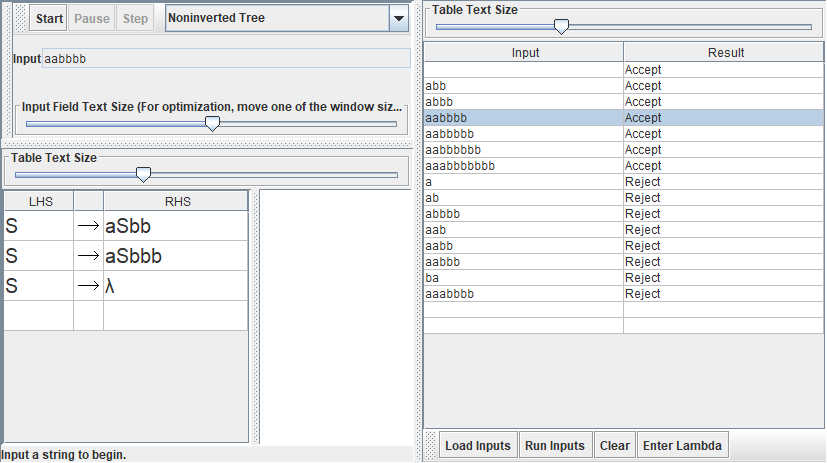
\includegraphics[width=0.95\textwidth]{Problem 1/Problem 1.png}
\caption{JFLAP verification of the grammar for Problem 1. The Multiple Run test demonstrates that the grammar correctly accepts strings where the number of $b$'s is between 2 and 3 times the number of $a$'s, and correctly rejects strings that violate this constraint. This confirms the grammar generates exactly the language $L = \{a^n b^m : 2n \le m \le 3n\}$.}
\label{fig:problem1}
\end{figure}

\subsection{Problem 2: CFG for $L = \{w \in \{a,b\}^* : n_a(w) = 2n_b(w)\}$}

\textbf{Context-Free Grammar:}

$$S \rightarrow aabS \mid abaS \mid baaS \mid \lambda$$

\textbf{Design Approach and Reasoning:}

The challenge is that the language allows arbitrary interleaving of $a$'s and $b$'s, as long as the final count maintains $n_a = 2n_b$. The grammar handles this through three recursive rules that each add exactly 2 $a$'s and 1 $b$ in different orderings. The rule $S \rightarrow aabS$ adds the pattern $aab$, while $S \rightarrow abaS$ adds the pattern $aba$, and $S \rightarrow baaS$ adds the pattern $baa$. These three rules cover all possible local arrangements of 2 $a$'s and 1 $b$, allowing the grammar to generate strings with arbitrary interleaving while maintaining the global 2:1 ratio. The base case $S \rightarrow \lambda$ generates the empty string.

\textbf{How the Grammar Works:}

Starting with $S$, we apply any combination of the three recursive rules. Each application adds a ``block'' of 2 $a$'s and 1 $b$ in some order, and the choice of which rule to apply determines the local ordering. We finish with $S \rightarrow \lambda$ to terminate the derivation. The result is a string where $n_a = 2n_b$ with arbitrary interleaving of the symbols.

\textbf{Test Cases and Correctness:}

\textbf{Accept Cases (strings in L):}
\begin{itemize}
\item $\lambda$ (empty string): $n_a=0, n_b=0$, satisfies $0 = 2(0)$ \checkmark
\item $aab$: $n_a=2, n_b=1$, satisfies $2 = 2(1)$ \checkmark
\item $aba$: $n_a=2, n_b=1$, satisfies $2 = 2(1)$ \checkmark
\item $baa$: $n_a=2, n_b=1$, satisfies $2 = 2(1)$ \checkmark
\item $aabaab$: $n_a=4, n_b=2$, satisfies $4 = 2(2)$ \checkmark
\item $aabbaa$: $n_a=4, n_b=2$, satisfies $4 = 2(2)$ \checkmark
\item $baaaab$: $n_a=4, n_b=2$, satisfies $4 = 2(2)$ \checkmark
\item $aaabaabaab$: $n_a=6, n_b=3$, satisfies $6 = 2(3)$ \checkmark
\end{itemize}

\textbf{Reject Cases (strings not in L):}
\begin{itemize}
\item $a$: $n_a=1, n_b=0$, violates $1 = 2(0)$ \texttimes
\item $b$: $n_a=0, n_b=1$, violates $0 = 2(1)$ \texttimes
\item $aa$: $n_a=2, n_b=0$, violates $2 = 2(0)$ \texttimes
\item $ab$: $n_a=1, n_b=1$, violates $1 = 2(1)$ \texttimes
\item $aaab$: $n_a=3, n_b=1$, violates $3 = 2(1)$ \texttimes
\item $aabb$: $n_a=2, n_b=2$, violates $2 = 2(2)$ \texttimes
\item $aaabb$: $n_a=3, n_b=2$, violates $3 = 2(2)$ \texttimes
\item $aaabbb$: $n_a=3, n_b=3$, violates $3 = 2(3)$ \texttimes
\end{itemize}

\textbf{Formal Proof of Correctness:}

\textbf{Claim:} $L(G) = \{w \in \{a,b\}^* : n_a(w) = 2n_b(w)\}$

\textbf{Proof:}

\textit{($\subseteq$ direction)} We prove that every string generated by $G$ satisfies $n_a = 2n_b$.

By induction on the number of derivation steps:

\textit{Base case:} If the derivation uses only $S \rightarrow \lambda$, then we generate $\lambda$ with $n_a(\lambda) = 0$ and $n_b(\lambda) = 0$. Since $0 = 2(0)$, the string satisfies the constraint.

\textit{Inductive hypothesis:} Assume that any string derived in $k$ or fewer steps satisfies $n_a = 2n_b$.

\textit{Inductive step:} Consider a derivation of length $k+1$. The first step must be one of: $S \rightarrow aabS$, $S \rightarrow abaS$, or $S \rightarrow baaS$.

For all three cases, the production adds 2 $a$'s and 1 $b$, then continues with $S$. If $S \Rightarrow^* w'$ where $n_a(w') = 2n_b(w')$ by the inductive hypothesis, then:
\begin{itemize}
\item $S \Rightarrow aabS \Rightarrow^* aabw'$: $n_a(aabw') = 2 + n_a(w') = 2 + 2n_b(w') = 2(1 + n_b(w')) = 2n_b(aabw')$ \checkmark
\item Similarly for $abaS$ and $baaS$
\end{itemize}

Therefore, every string in $L(G)$ satisfies $n_a = 2n_b$.

\textit{($\supseteq$ direction)} We prove that every string with $n_a = 2n_b$ can be generated by $G$.

By strong induction on the length of the string:

\textit{Base case:} The empty string $\lambda$ has $n_a = n_b = 0$, so $0 = 2(0)$. It is generated by $S \rightarrow \lambda$.

\textit{Inductive hypothesis:} Assume that every string of length at most $k$ with $n_a = 2n_b$ can be generated by $G$.

\textit{Inductive step:} Let $w$ be a string of length $k+1$ with $n_a(w) = 2n_b(w)$. Since $|w| > 0$ and $n_a(w) = 2n_b(w)$, we must have $n_b(w) \ge 1$ (otherwise $n_a(w) = 0$ and $w = \lambda$).

Consider the first occurrence of $b$ in $w$. Let $w = x b y$ where $x \in \{a\}^*$ and $b$ is the first $b$ in $w$.

Since $n_a(w) = 2n_b(w)$ and $n_b(w) \ge 1$, we have $n_a(w) \ge 2$. Therefore, $|x| \ge 2$.

We can write $x = aa x'$ where $x' \in \{a\}^*$. Then $w = aa b y'$ where $y' = x' y$.

Let $w' = x' y$. Then:
\begin{itemize}
\item $n_a(w') = n_a(w) - 2 = 2n_b(w) - 2 = 2(n_b(w) - 1) = 2n_b(w')$
\item $|w'| = |w| - 3 < k+1$
\end{itemize}

By the inductive hypothesis, $w'$ can be generated by $G$. Therefore:
$$S \Rightarrow aabS \Rightarrow^* aabw' = w$$

Thus, $w$ can be generated by $G$.

Therefore, $L(G) = \{w \in \{a,b\}^* : n_a(w) = 2n_b(w)\}$. $\square$

\begin{figure}[H]
\centering
\includegraphics[width=0.95\textwidth]{Problem 2/Problem 2.png}
\caption{JFLAP verification of the grammar for Problem 2. The Multiple Run test demonstrates that the grammar correctly accepts strings with arbitrary interleaving of $a$'s and $b$'s where $n_a = 2n_b$, and correctly rejects strings that violate the 2:1 ratio. This confirms the grammar handles all possible orderings while maintaining the constraint.}
\label{fig:problem2}
\end{figure}

\section{Section 5.2: Derivation Trees and Ambiguity}

\subsection{Problem 3: Derivation Tree for $(a+b)*c+d$}

\textbf{Grammar Rules (Modified Example 5.12):}

$$\begin{aligned}
E &\rightarrow E+T \mid T \\
T &\rightarrow T*F \mid F \\
F &\rightarrow (E) \mid I \\
I &\rightarrow a \mid b \mid c \mid d
\end{aligned}$$

\textbf{Precedence Hierarchy:}
\begin{itemize}
\item \textbf{Lowest Precedence:} Addition ($+$) - handled by $E$ rules
\item \textbf{Medium Precedence:} Multiplication ($*$) - handled by $T$ rules
\item \textbf{Highest Precedence:} Parentheses and identifiers - handled by $F$ and $I$ rules
\end{itemize}

\textbf{Design Approach and Reasoning:}

This grammar enforces correct operator precedence through its hierarchical structure. The expression level ($E$) handles addition, the lowest precedence operator. The term level ($T$) handles multiplication, which binds tighter than addition. The factor level ($F$) handles parentheses (highest precedence) and atomic identifiers. Finally, the identifier level ($I$) represents the terminal symbols (variables). The grammar ensures that multiplication is performed before addition, and parenthesized expressions are evaluated first.

\textbf{Leftmost Derivation Sequence:}

For the string $(a+b)*c+d$:

$$\begin{aligned}
E &\Rightarrow E+T \\
&\Rightarrow T+T \\
&\Rightarrow T*F+T \\
&\Rightarrow F*F+T \\
&\Rightarrow (E)*F+T \\
&\Rightarrow (E+T)*F+T \\
&\Rightarrow (T+T)*F+T \\
&\Rightarrow (F+T)*F+T \\
&\Rightarrow (I+T)*F+T \\
&\Rightarrow (a+T)*F+T \\
&\Rightarrow (a+F)*F+T \\
&\Rightarrow (a+I)*F+T \\
&\Rightarrow (a+b)*F+T \\
&\Rightarrow (a+b)*I+T \\
&\Rightarrow (a+b)*c+T \\
&\Rightarrow (a+b)*c+F \\
&\Rightarrow (a+b)*c+I \\
&\Rightarrow (a+b)*c+d
\end{aligned}$$

\textbf{Derivation Tree Structure:}

The parse tree has $E$ as the root (the start symbol). The first split is $E \rightarrow E+T$, representing the outermost addition operation. The left subtree derives the expression $(a+b)*c$ from the left $E$. This $E$ reduces to $T$ (no addition at this level), which then expands via $T \rightarrow T*F$ to represent multiplication. The left $T$ derives $(a+b)$ through parentheses, while the right $F$ derives $c$. The right subtree of the root derives the term $d$ from the right $T$.

The tree structure correctly shows that the outermost operation is addition ($+$), with the left operand being $(a+b)*c$ (demonstrating that multiplication has higher precedence) and the right operand being $d$. Inside the parentheses, $a+b$ is correctly parsed as addition. This enforces the evaluation order: $((a+b)*c)+d$.

\begin{figure}[H]
\centering
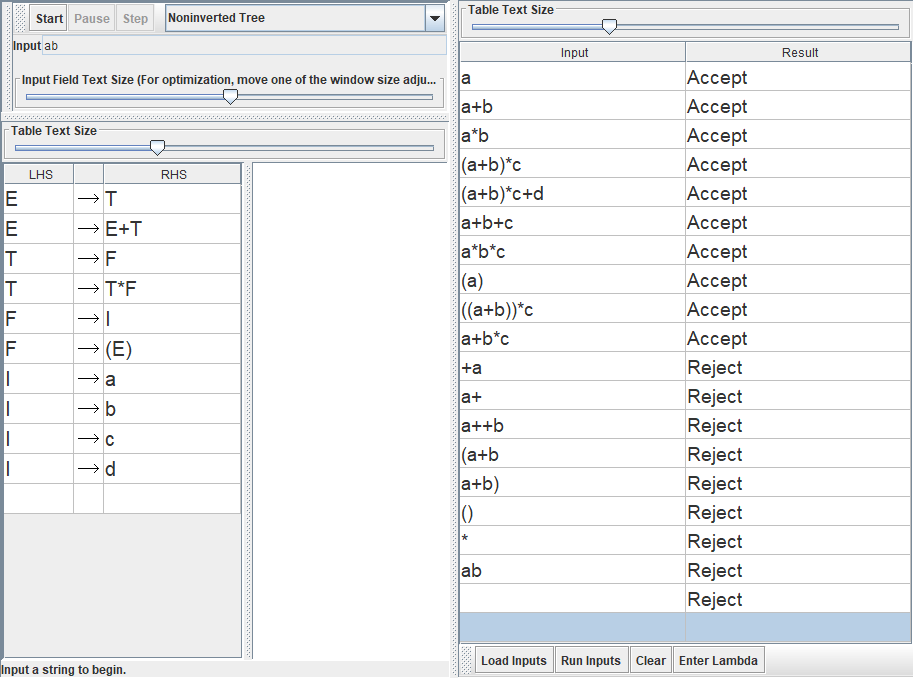
\includegraphics[width=0.95\textwidth]{Problem 3/Problem 3.png}
\caption{JFLAP verification that the expression grammar correctly parses arithmetic expressions. The test results confirm the grammar accepts well-formed expressions with proper operator precedence and rejects malformed expressions with syntax errors.}
\label{fig:problem3_tests}
\end{figure}

\begin{figure}[H]
\centering
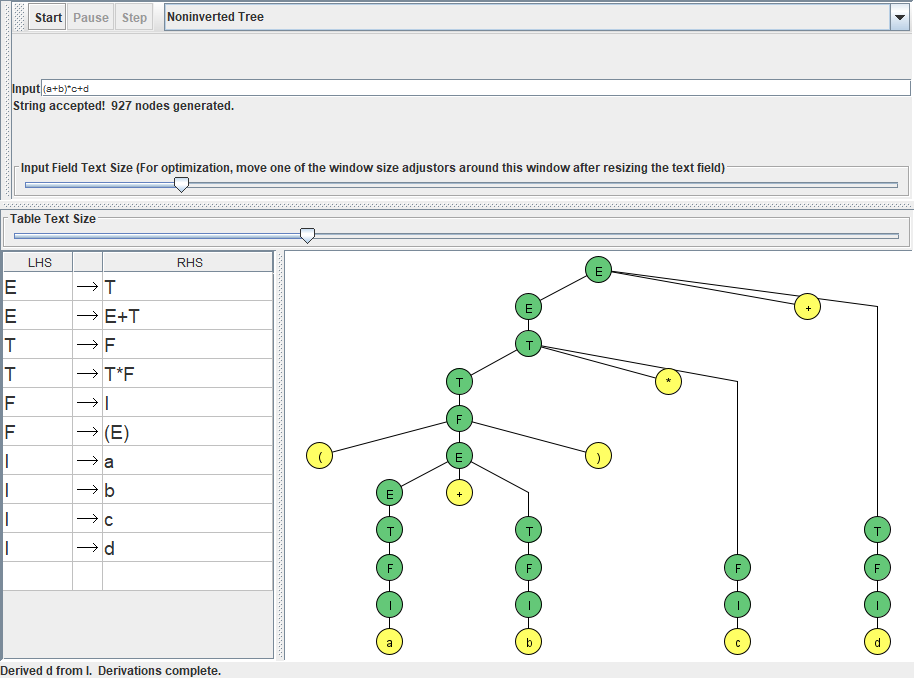
\includegraphics[width=0.95\textwidth]{Problem 3/Problem 3 B.png}
\caption{Complete derivation tree for $(a+b)*c+d$ generated by JFLAP's Brute Force Parse. The tree structure visually confirms that the grammar enforces correct operator precedence: the outermost operation is addition, with $(a+b)*c$ as the left operand (showing multiplication binds tighter than addition), and $d$ as the right operand. The parentheses force $a+b$ to be evaluated first.}
\label{fig:problem3_tree}
\end{figure}

\subsection{Problem 4: Ambiguity Proof}

\textbf{Grammar:} $S \rightarrow aSb \mid SS \mid \lambda$

\subsubsection{Part I: Proving the Grammar is Ambiguous}

\textbf{Definition:} A grammar is ambiguous if there exists at least one string in the language that has two or more distinct parse trees (or equivalently, two or more distinct leftmost derivations).

\textbf{Proof Strategy:} We demonstrate ambiguity by exhibiting a string with two distinct parse trees.

\textbf{Witness String:} $w = aabb$

\textbf{Derivation 1 (Using $S \rightarrow aSb$ first):}

$$\begin{aligned}
S &\Rightarrow aSb \\
&\Rightarrow aaSbb \\
&\Rightarrow a\lambda bb \\
&\Rightarrow aabb
\end{aligned}$$

\textbf{Parse Tree 1 Structure:}

This tree represents a \textbf{nested structure}: the string is parsed as $a(ab)b$, where the inner $ab$ is wrapped by an outer $a$ and $b$.

\textbf{Derivation 2 (Using $S \rightarrow SS$ first):}

$$\begin{aligned}
S &\Rightarrow SS \\
&\Rightarrow aSbS \\
&\Rightarrow a\lambda bS \\
&\Rightarrow abS \\
&\Rightarrow abaSb \\
&\Rightarrow aba\lambda b \\
&\Rightarrow aabb
\end{aligned}$$

\textbf{Parse Tree 2 Structure:}

This tree represents a \textbf{concatenation structure}: the string is parsed as $(ab)(ab)$, where two independent $ab$ substrings are concatenated.

\textbf{Conclusion:} Since the string $aabb$ has two distinct parse trees with different structural interpretations, the grammar $G_A: S \rightarrow aSb \mid SS \mid \lambda$ is \textbf{ambiguous}.

\begin{figure}[H]
\centering
\includegraphics[width=0.95\textwidth]{Problem 4/Ambiguous Grammar Tree 1 (aSb First)-Tests-BlowUp.png}
\caption{JFLAP verification of the ambiguous grammar $S \rightarrow aSb \mid SS \mid \lambda$. The test results confirm the grammar correctly generates the language of balanced parentheses, accepting strings where $n_a = n_b$ with proper nesting, and rejecting unbalanced strings.}
\label{fig:problem4_tests}
\end{figure}

\begin{figure}[H]
\centering
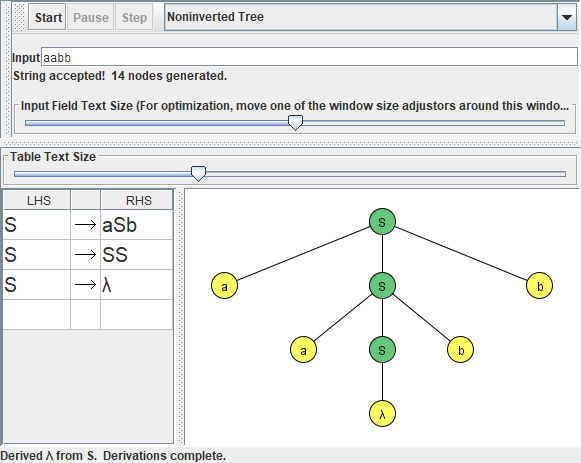
\includegraphics[width=0.7\textwidth]{Problem 4/Ambiguous Grammar Tree 1 (aSb First).png}
\caption{First parse tree for $aabb$ generated by JFLAP using the derivation $S \Rightarrow aSb \Rightarrow aaSbb \Rightarrow aabb$. This tree represents a \textbf{nested structure} where the string is parsed as $a(ab)b$, with the inner $ab$ wrapped by an outer $a$ and $b$. The existence of this tree is part of the proof that the grammar is ambiguous.}
\label{fig:problem4_tree1}
\end{figure}

\begin{figure}[H]
\centering
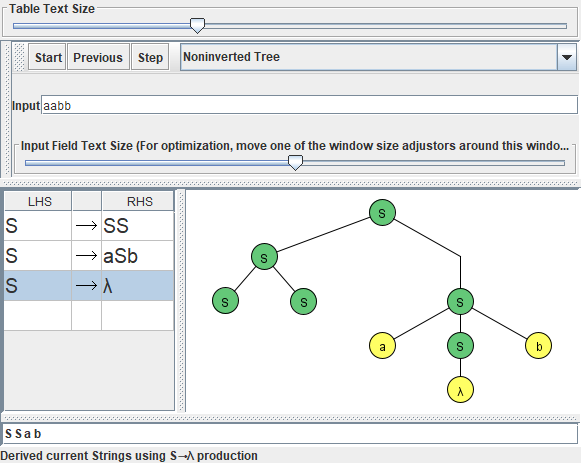
\includegraphics[width=0.7\textwidth]{Problem 4/Ambiguous Grammar Tree 2 (SS First).png}
\caption{Second parse tree for $aabb$ generated by JFLAP using the derivation $S \Rightarrow SS \Rightarrow aSbS \Rightarrow \cdots \Rightarrow aabb$. This tree represents a \textbf{concatenation structure} where the string is parsed as $(ab)(ab)$, with two independent $ab$ substrings concatenated. Since $aabb$ has two structurally different parse trees, this proves the grammar is ambiguous.}
\label{fig:problem4_tree2}
\end{figure}

\subsubsection{Part II: Proving the Language is NOT Inherently Ambiguous}

\textbf{Definition:} A language is inherently ambiguous if every grammar that generates it is ambiguous. Conversely, a language is NOT inherently ambiguous if there exists at least one unambiguous grammar that generates it.

\textbf{Proof Strategy:} We construct an unambiguous grammar that generates the same language as $G_A$.

\textbf{Language Analysis:}

First, we determine what language $G_A$ generates. The grammar has three rules:
\begin{itemize}
\item $S \rightarrow aSb$: Adds matching $a$ and $b$ on the outside
\item $S \rightarrow SS$: Concatenates two strings from the language
\item $S \rightarrow \lambda$: Generates the empty string
\end{itemize}

By analyzing the grammar, we can show that $L(G_A) = \{w \in \{a,b\}^* : n_a(w) = n_b(w) \text{ and every prefix has } n_a \ge n_b\}$. This is the language of \textbf{balanced parentheses} (if we think of $a$ as ``('' and $b$ as ``)'').

\textbf{Unambiguous Grammar:}

$$G_U: S \rightarrow aSbS \mid \lambda$$

\textbf{Why $G_U$ is Unambiguous:}

The grammar $G_U$ has only two rules, and the structure is carefully designed:
\begin{enumerate}
\item $S \rightarrow aSbS$: This rule adds an $a$, then recursively generates a balanced substring, then adds a $b$, then recursively generates another balanced substring
\item $S \rightarrow \lambda$: Base case
\end{enumerate}

For any string in the language, there is exactly one way to parse it:
\begin{itemize}
\item The first $a$ in the string must be matched with its corresponding $b$ (the first $b$ that closes the balanced prefix)
\item This uniquely determines where to split the string
\item The grammar enforces a \textbf{canonical parsing} where each $a$ is immediately followed by its matching balanced substring before the closing $b$
\end{itemize}

\textbf{Proof that $L(G_U) = L(G_A)$:}

We need to show that both grammars generate the same language.

\textbf{($L(G_U) \subseteq L(G_A)$):} Every string generated by $G_U$ can be generated by $G_A$:
\begin{itemize}
\item $\lambda$ is generated by both
\item If $G_U$ generates $aSbS$, we can use $G_A$ to generate $aSb$ (from the first part) and $S$ (from the second part), then concatenate using $SS$
\end{itemize}

\textbf{($L(G_A) \subseteq L(G_U)$):} Every string generated by $G_A$ can be generated by $G_U$:
\begin{itemize}
\item This requires showing that the concatenation rule $SS$ in $G_A$ can be simulated by the $aSbS$ rule in $G_U$
\item The key insight is that any balanced string can be decomposed into a form where the first $a$ is matched with a specific $b$, and the remaining parts are balanced
\end{itemize}

\textbf{Verification with JFLAP:}

The screenshots show that $G_U$ accepts the same set of test strings as $G_A$:
\begin{itemize}
\item Both accept: $\lambda$, $ab$, $aabb$, $abab$, $aaabbb$, etc.
\item Both reject: $a$, $b$, $ba$, $abb$, $aab$, etc.
\end{itemize}

\textbf{Conclusion:} Since we have constructed an unambiguous grammar $G_U$ that generates the same language as $G_A$, the language $L(G_A)$ is \textbf{NOT inherently ambiguous}.

\begin{figure}[H]
\centering
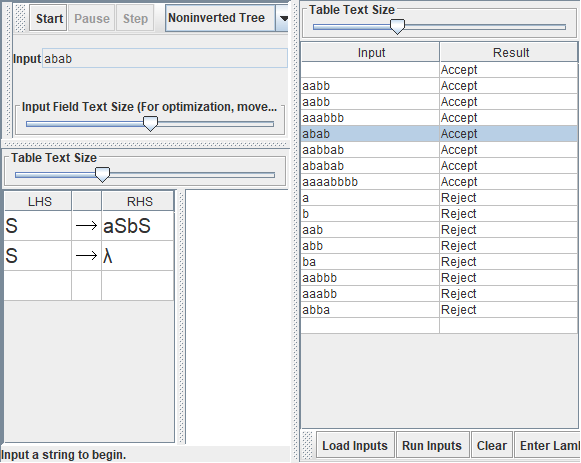
\includegraphics[width=0.95\textwidth]{Problem 4/Unambiguous Grammer-Tests.png}
\caption{JFLAP verification of the unambiguous grammar $S \rightarrow aSbS \mid \lambda$. The test results show this grammar accepts and rejects the exact same strings as the ambiguous grammar, proving both grammars generate the same language. This is crucial evidence that the language is not inherently ambiguous.}
\label{fig:problem4_unambiguous_tests}
\end{figure}

\begin{figure}[H]
\centering
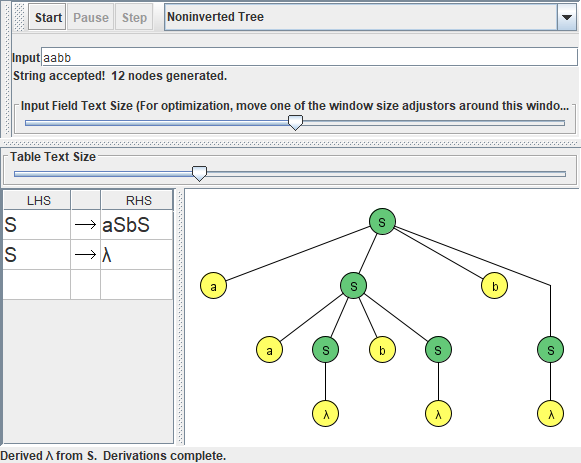
\includegraphics[width=0.7\textwidth]{Problem 4/Unambiguous Grammar-Tree.png}
\caption{Parse tree for $aabb$ using the unambiguous grammar $S \rightarrow aSbS \mid \lambda$. Unlike the ambiguous grammar which produced two different parse trees for this string, the unambiguous grammar produces only one parse tree. This demonstrates that the grammar enforces a canonical parsing strategy, completing the proof that the language is not inherently ambiguous.}
\label{fig:problem4_unambiguous_tree}
\end{figure}

\textbf{Summary:}
\begin{itemize}
\item \textbf{Part I:} The grammar $S \rightarrow aSb \mid SS \mid \lambda$ is ambiguous (proven by exhibiting two parse trees for $aabb$)
\item \textbf{Part II:} The language generated by this grammar is not inherently ambiguous (proven by constructing the unambiguous grammar $S \rightarrow aSbS \mid \lambda$)
\end{itemize}

\subsection{Problem 5: Unambiguous Single-Production Grammars}

\textbf{Theorem Statement:}

\textbf{Theorem:} Let $G = (V, T, S, P)$ be a context-free grammar such that each variable $A \in V$ appears on the left-hand side of at most one production in $P$. Then $G$ is unambiguous.

\textbf{Proof:}

We prove this directly by showing that every string $w \in L(G)$ has a unique derivation tree.

We proceed by strong induction on the number of derivation steps required to generate $w$.

\textbf{Base Case ($n = 1$):}

If $w$ is derived in one step, the derivation is $S \rightarrow w$. Since $S$ has at most one production in $P$, this derivation (and its resulting tree) is uniquely determined.

\textbf{Inductive Hypothesis:}

Assume that for all strings derivable in $k$ or fewer steps ($k \ge 1$), the derivation tree is unique.

\textbf{Inductive Step (Conclusion):}

Consider a string $w$ derived in $k + 1$ steps. The derivation must begin with the first production:

$$S \Rightarrow \alpha$$

where $\alpha = \alpha_1 \alpha_2 \dots \alpha_m$. Since the variable $S$ appears on the left side of at most one production, this initial step $S \rightarrow \alpha$ is uniquely determined.

The final string $w$ is partitioned as $w = w_1 w_2 \dots w_m$. For any $\alpha_i \in V$ (a variable), $w_i$ is derived from $\alpha_i$ in fewer than $k+1$ steps. Since each variable $\alpha_i$ has at most one production, the derivation tree for $w_i$ from $\alpha_i$ is unique by the inductive hypothesis.

Since:
\begin{enumerate}
\item The first step ($S \rightarrow \alpha$) is unique.
\item Every subsequent subtree derived from $\alpha_i$ is unique.
\end{enumerate}

The entire derivation tree for $w$ is uniquely determined.

By the principle of mathematical induction, every string in $L(G)$ has a unique derivation tree.

Therefore, the grammar $\mathbf{G}$ is unambiguous. $\square$

\textbf{Intuitive Explanation:}

The key insight of this proof is that the constraint ``no variable appears on the left side of more than one production'' eliminates all sources of ambiguity:

\begin{enumerate}
\item \textbf{No choice at any step:} When deriving from a variable $A$, there is at most one production $A \rightarrow \beta$ to apply
\item \textbf{Deterministic derivation:} The derivation process becomes deterministic---at each step, there is only one possible production to apply
\item \textbf{Unique parse tree:} Since every derivation step is forced, there can be only one parse tree for any string
\end{enumerate}

This is a very restrictive condition on grammars (most useful grammars have multiple productions for the same variable), but it guarantees unambiguity.

\textbf{Example:}

Consider the grammar:
$$\begin{aligned}
S &\rightarrow AB \\
A &\rightarrow a \\
B &\rightarrow b
\end{aligned}$$

Each variable ($S$, $A$, $B$) appears on the left side of exactly one production. For the string $ab$:
\begin{itemize}
\item Must start with $S \rightarrow AB$ (only production for $S$)
\item Must derive $A \rightarrow a$ (only production for $A$)
\item Must derive $B \rightarrow b$ (only production for $B$)
\item Result: unique derivation tree
\end{itemize}

This grammar satisfies the theorem's hypothesis and is indeed unambiguous.

\end{document}
